\documentclass[conference]{IEEEtran}
\usepackage{cite}
\usepackage{amsmath,amssymb,amsfonts}
\usepackage{graphicx}
\usepackage{textcomp}
\usepackage{xcolor}
\usepackage{listings}
\usepackage{booktabs}
\usepackage{array}
\usepackage{url}

\lstset{basicstyle=\ttfamily\scriptsize, columns=fullflexible, frame=single, aboveskip=4pt, belowskip=4pt,
	morekeywords={edition,enemy,mode,player,arena,waves,wave,drops,win,lose,when,split,into,on,pop,contact}}

\begin{document}

\title{Rango Unchained: A Model-Driven Product Line of Game Modes}

\author{\IEEEauthorblockN{Aleksander Kvelland}
\and
\IEEEauthorblockN{Ferdinand Fremming}
\and
\IEEEauthorblockN{Fredrik L.}
\and
\and
\IEEEauthorblockN{Marius Norheim Engebretsen}
\and
\IEEEauthorblockN{Eirik Johan Andreassen}
}

\maketitle

\begin{abstract}
We turn the game modes of Rango Unchained, a libGDX clone of Bubble Trouble, into a software product
line. An edition of the game is described in a textual domain-specific language built on an Ecore
metamodel, validated in an Xtext editor, and generated into the game as Java classes, level resources
and product configuration. This report explains the idea and
motivation, and the main design choices in the metamodel, the concrete syntax, the generator and the
build.
\end{abstract}

\begin{IEEEkeywords}
model-driven engineering, domain-specific languages, software product lines, EMF, Xtext, code
generation, game development
\end{IEEEkeywords}

\section{Idea and Motivation}
Rango Unchained is a 2D arcade game built with libGDX~\cite{libgdx} in an earlier course: the player
pops bouncing enemies with a tongue, and popped enemies split into smaller ones. In the original game,
you played a campaign with different JSON levels you loaded. How enemies split, what they do to the player, what
drops, and when a round is won or lost were hard-coded. Adding a mode meant editing Java in several
places. Yet these are exactly the things in which one mode differs from another, and they are what a
game designer wants to experiment with.

We therefore chose \emph{game modes} as the single variability aspect and treat the game as a
software product line~\cite{spl}. One \emph{edition} (a product) is a set of game modes and the
building blocks they share. We model the aspect in its entirety: everything that makes one mode
differ from another is in the metamodel and reaches the game; nothing else is. Rendering, sound,
animation, menus, multiplayer and the user system do not vary between modes and stay out of the
language. The campaign is modelled as a game mode of several levels, so single player is no longer a
separate system next to the modes.

The solution is a chain of Eclipse tools. A designer writes an edition in a \texttt{.rango} file.
Xtext parses it into an instance of the Ecore metamodel, which is checked by OCL and Java
constraints. Xtend templates then generate the edition into the game, and the game's own Gradle
build turns it into a playable product. All of it is built headless with Maven/Tycho.

\section{Metamodel}
The metamodel (EMF~\cite{emf}, \texttt{gamemode.ecore}, 42 classes, 9 of them abstract, Fig.~\ref{fig:metamodel})
has an \texttt{Edition} as root. It \emph{contains} reusable building blocks (enemy types, power-ups,
player profiles, default drop tables, difficulties) and the game modes made from them, which
\emph{reference} the blocks.

\begin{figure*}[t]
\centerline{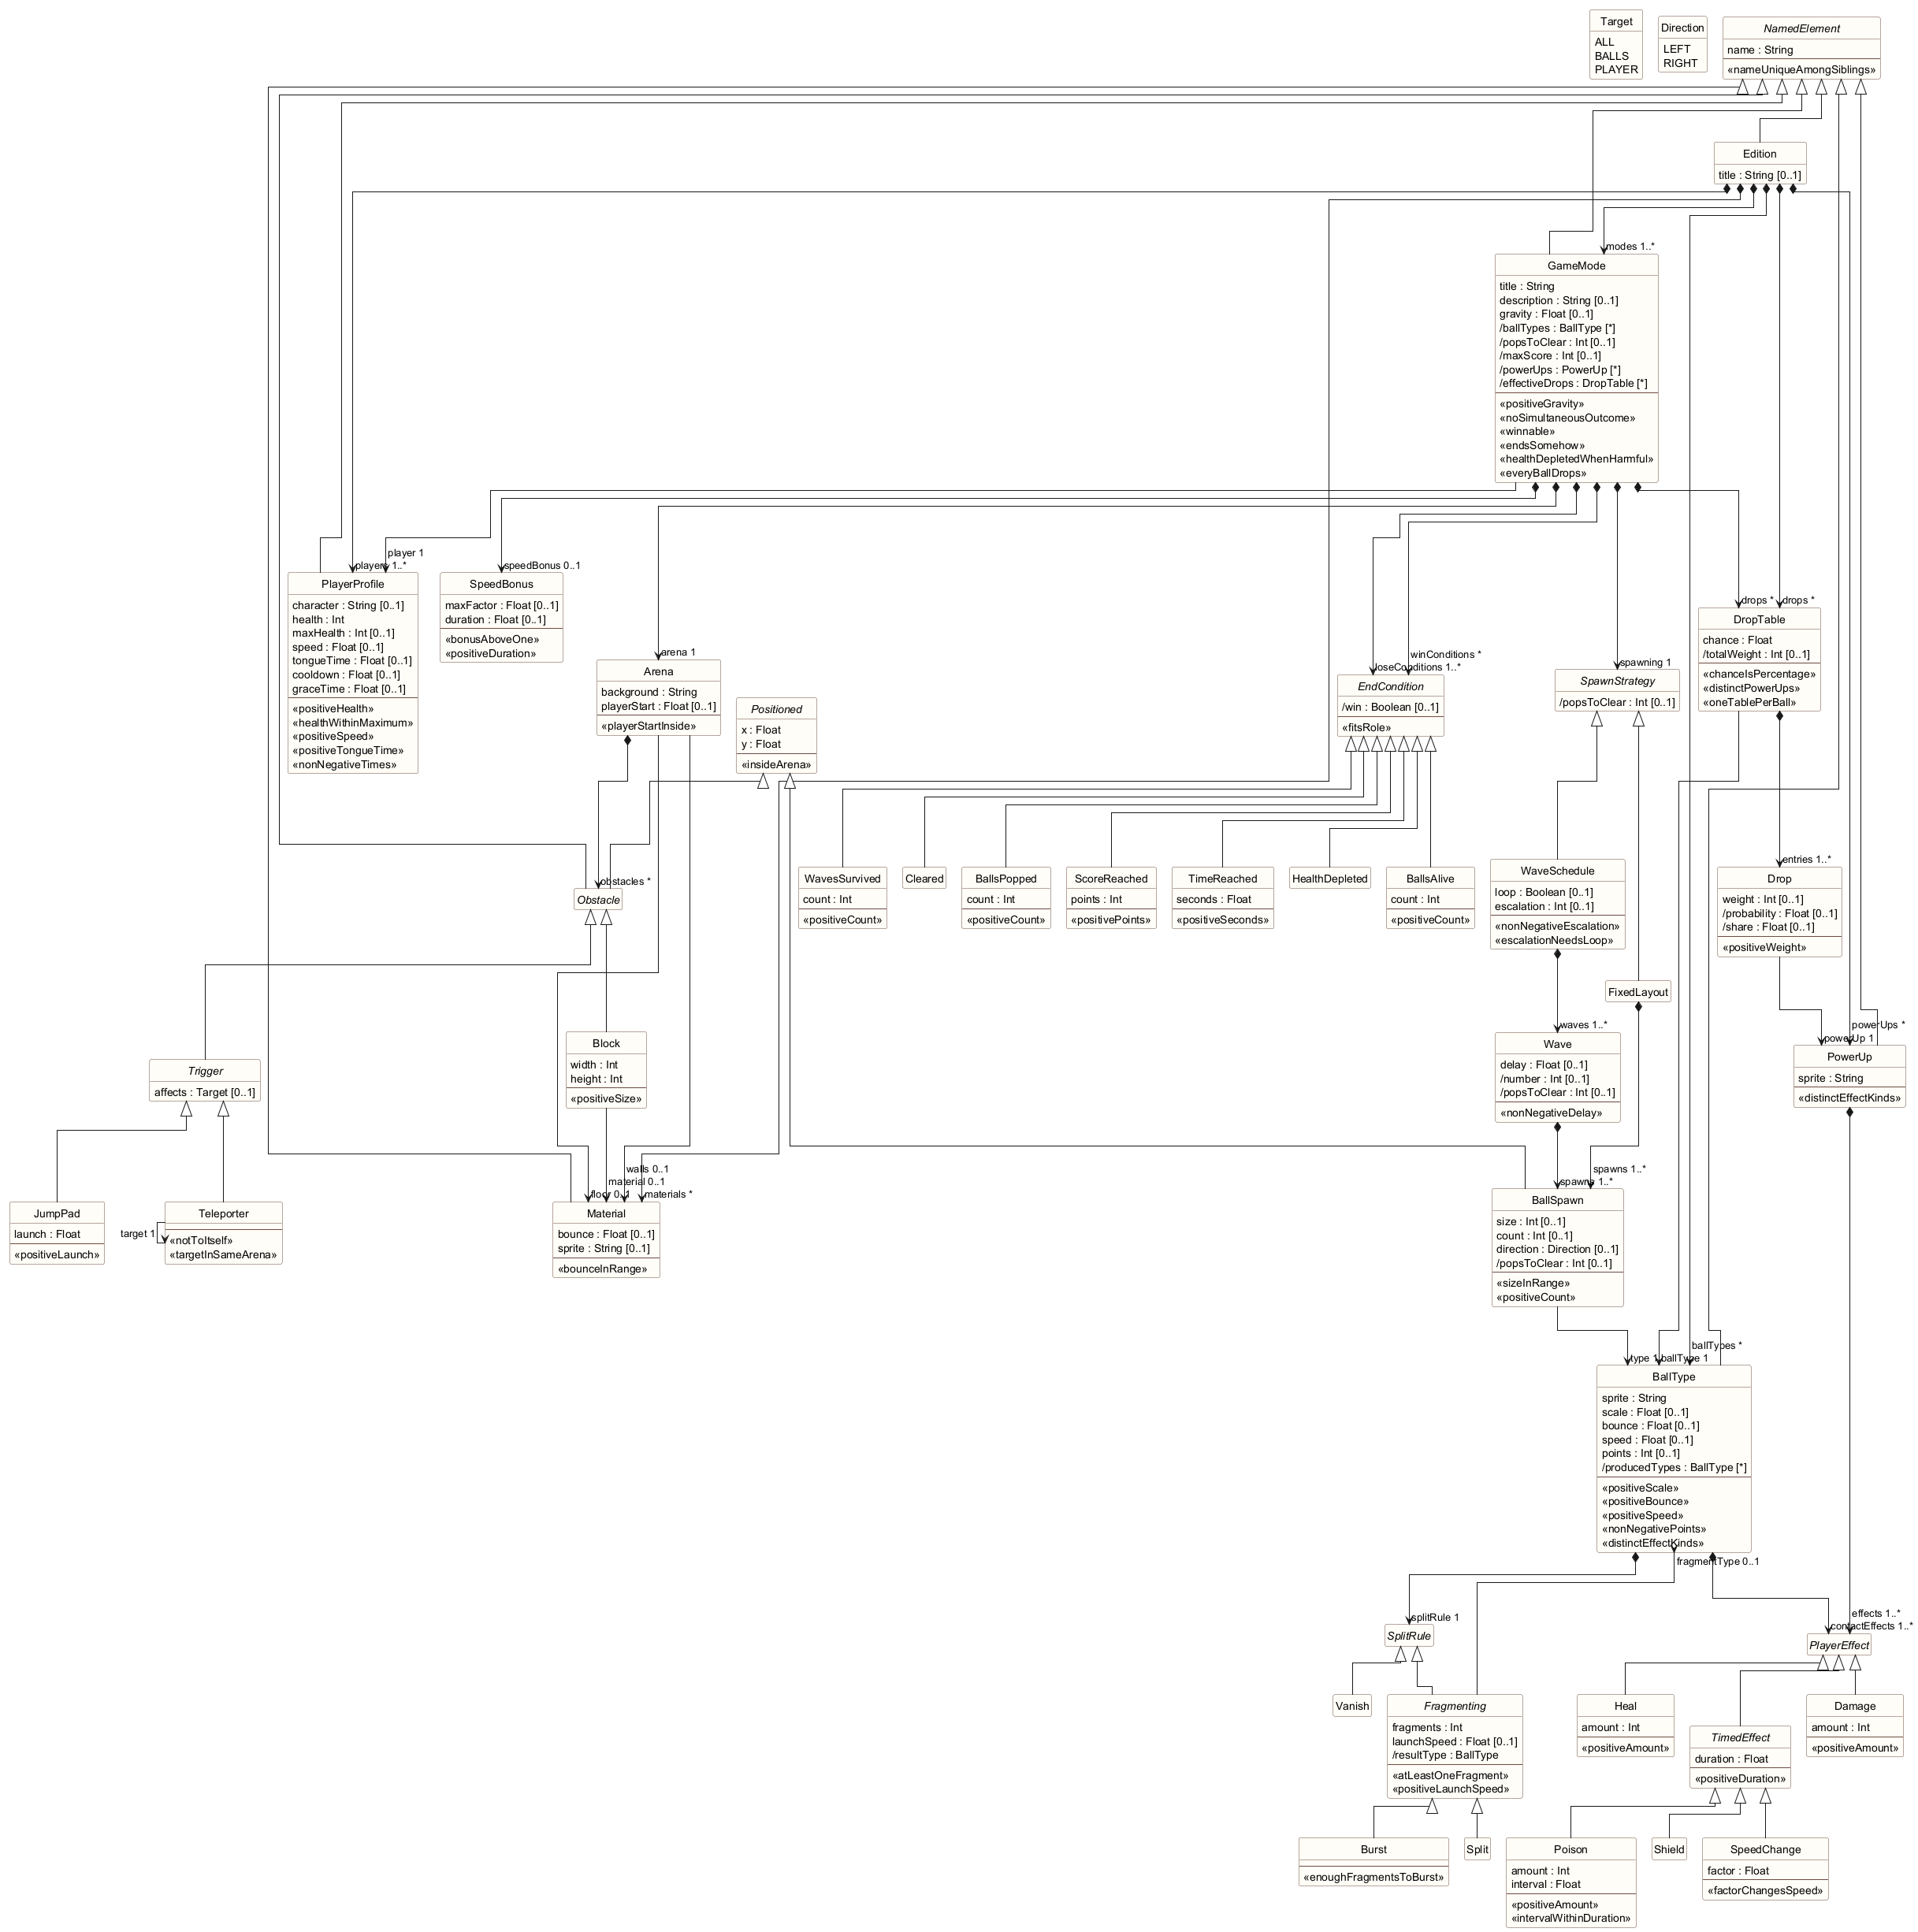
\includegraphics[width=0.7\textwidth]{../metamodel.png}}
\caption{Class diagram of the metamodel, generated from \texttt{gamemode.ecore}.}
\label{fig:metamodel}
\end{figure*}

\subsection{Library elements with behaviour, not enumerations}
Our draft listed the enemies of the game as an enum. Following the feedback, an \texttt{EnemyType} is
now defined by its tuning, the \texttt{SplitRule} it contains, and the \texttt{PlayerEffect}s it has
on contact. ``Cactus'' or ``Bomb'' are instances, so a new enemy needs no change to the metamodel or
the game. Variation that carries different data is modelled as subclasses of an abstract class:
\texttt{SplitRule} is \texttt{Vanish} or \texttt{Split}; \texttt{PlayerEffect} is \texttt{Damage},
\texttt{Heal} or the abstract \texttt{TimedEffect} (\texttt{Shield}, \texttt{SpeedChange},
\texttt{Poison}). Effects are shared by enemy contacts and power-ups, so ``poison'' means the same in
both places. Enums are kept for closed sets of labels without behaviour (\texttt{Direction},
\texttt{DifficultyTier}, \texttt{ModifierTarget}).

\subsection{Modes, levels and end conditions}
A \texttt{GameMode} contains one or more \texttt{Level}s. Each level contains an \texttt{Arena}
(obstacles: \texttt{Block}s and \texttt{Trigger}s, i.e.\ \texttt{JumpPad}s and \texttt{Teleporter}s)
and a \texttt{SpawnStrategy}, which is a \texttt{FixedLayout} or a \texttt{WaveSchedule} that can loop
and escalate. Obstacles and spawns share the abstract \texttt{Positioned}.

\texttt{EndCondition} has seven subclasses (\texttt{Cleared}, \texttt{TimeReached},
\texttt{ScoreReached}, \ldots). The same class can win or lose a round: \texttt{TimeReached} is
``survive 60\,s'' as a win and a time limit as a loss. We do not store a \texttt{win} flag; the role
is given by the containing list (\texttt{winConditions} or \texttt{loseConditions}) and exposed as a
derived feature.

\subsection{Drop tables and difficulty}
A \texttt{DropTable} references one enemy type and contains weighted \texttt{Drop}s that reference
power-ups. Drop rates thus depend on which enemy is popped and on the mode: a mode's own tables
replace the edition's defaults. Which tables apply is derived (\texttt{effectiveDrops}) rather than
copied into each mode.

An edition can define up to three \texttt{Difficulty}s, one per tier. A difficulty contains
\texttt{Modifier}s, each multiplying one kind of modelled value (enemy speed, points, player health
and speed, drop chance, wave delay) by a factor in every mode. Values without a modifier are played
as modelled, so the tiers tune an edition without copying its modes.

\subsection{Derived features and constraints}
We never store what can be derived. Derived features (Java, \texttt{GamemodeDerivations}) include the
enemy types of a mode (recursively through split rules), the pops needed to clear a level, the
maximum score, and the probability that a pop drops a given power-up. The generator, the editor
hovers and the constraints all reuse them.

Constraints are domain rules, not artificial limits. Single-object invariants are in OCL in the Ecore
model (e.g.\ a drop chance is a percentage, a teleporter does not lead to itself). Rules spanning
several objects are in Java with stable diagnostic codes. An example
is \texttt{winnable}: every win condition can be met in every level, so ``all enemies cleared'' with
looping waves, or a score above the derived maximum, is an error. Others are \texttt{endsSomehow},
\texttt{noSimultaneousOutcome} (a round cannot be won and lost by the same event), and
\texttt{everyEnemyDrops}.

\section{Concrete Syntax and Editor}
The Xtext~\cite{xtext} grammar \emph{imports} the hand-made metamodel instead of generating one, so all OCL and Java
constraints and derived features apply in the editor. The syntax is customised to read like a game
description, with units, percentages, positions and counts:

\begin{lstlisting}
enemy Mine {
  sprite "Enemy/Bomb.png"
  points 30
  on pop: split into 4 Weed
  on contact: damage 2
}
mode TimeAttack "Time Attack" {
  player Sprinter
  waves looping escalate by 1 {
    wave { 2 * Tumbleweed size 3 at (50%, 80%) }
  }
  drops { Mine 50% { Rush weight 3, Heart } }
  win when score reaches 1500
  lose when time reaches 90 s or health depleted
}
\end{lstlisting}

Beyond the generated defaults, the editor has scoping (a teleporter can only target one in its own
arena), quick fixes keyed on the constraint codes, hovers that show derived facts, an outline with
summaries, content assist for the game's images, templates, a formatter, and a command that generates
into a chosen game folder and refuses invalid models.

\section{Generation and Runtime}
We split the target code in two. A small \emph{hand-written runtime} in the game
(\texttt{GameModeDefinition}, \texttt{ModeSession}, contact rules and level progress) implements what
is the same for all modes: timers, timed effects, wave scheduling and statistics. The \emph{Xtend
generator} writes what varies, so the templates only map the model to code and contain no domain
logic. For each edition it produces:
\begin{itemize}
\item one Java class per mode: split rules become \texttt{split} calls with the derived spacing,
effects become player calls, drop tables become chance rolls and weighted picks per enemy, waves
become spawn schedules, and end conditions become the expressions of \texttt{isWon} and
\texttt{isLost};
\item one JSON arena per level, in the game's existing level format;
\item the edition class (product name, mode order, difficulty modifiers) read by the menu and the
desktop launcher, and the Android \texttt{edition.xml}.
\end{itemize}
Output is deterministic, carries a ``do not edit'' header, and stale files are removed, so a mode
deleted from the model disappears from the game. Hooks in the existing game are kept small: factories
read enemy kinds and player tuning from the mode, and the menu lists the edition's modes.

\section{Examples and Validation}
Three structurally different editions show the range of the product line. \emph{Classic} has a
five-level campaign and an endless mode with looping waves, teleporters, edition-wide drop tables and
three difficulty tiers. \emph{Arcade} has five short modes with two player profiles, a speed bonus,
mode-specific drop tables and different win conditions (score, pops, time, waves). \emph{Hardcore}
has one mode, a one-heart player, chained splits and no difficulty tiers. A test checks that the
three together use every concrete class, feature and enum literal of the metamodel. Each constraint
has a test that breaks exactly that rule on a valid fixture, and generator tests check the produced
code.

\section{Build and Packaging}
Everything is built headless with Maven/Tycho against a pinned Eclipse 2026-06 target platform: the
model, the language (MWE2 regeneration on every build), the editor, the tests, an Eclipse feature
and a p2 update site. The profile \texttt{-Pgame -Dedition=arcade} generates an example into the game
and builds it with Gradle, so deriving a product is one command. The repository README documents
setup and use in detail.

\section{Discussion}
Modelling behaviour (split rules, effects, end conditions) instead of named entities made the
metamodel smaller than an enumeration-based design, and lets a designer create enemies and modes the
original game never had. The cost is a runtime that must interpret every combination, which we keep
honest by generating and playing all three examples. Gameplay balance cannot be checked by
constraints; we only guarantee that every mode is winnable, losable and ends.

\begin{thebibliography}{00}
\bibitem{spl} K.~Pohl, G.~B\"ockle, and F.~van~der~Linden, \emph{Software Product Line Engineering:
Foundations, Principles and Techniques}. Berlin: Springer, 2005.
\bibitem{emf} D.~Steinberg, F.~Budinsky, M.~Paternostro, and E.~Merks, \emph{EMF: Eclipse Modeling
Framework}, 2nd~ed. Boston: Addison-Wesley, 2009.
\bibitem{xtext} L.~Bettini, \emph{Implementing Domain-Specific Languages with Xtext and Xtend},
2nd~ed. Birmingham: Packt, 2016.
\bibitem{libgdx} libGDX, ``libGDX: Cross-platform Java game development framework.'' [Online].
Available: \url{https://libgdx.com/}
\end{thebibliography}

\end{document}
